\documentclass{article}


% if you need to pass options to natbib, use, e.g.:
%     \PassOptionsToPackage{numbers, compress}{natbib}
% before loading neurips_2023


% ready for submission
% \usepackage{neurips_2023, hypertype}


% to compile a preprint version, e.g., for submission to arXiv, add add the
% [preprint] option:
\usepackage[preprint]{neurips_2023}
\usepackage{hypertype}


% to compile a camera-ready version, add the [final] option, e.g.:
%     \usepackage[final]{neurips_2023}


% to avoid loading the natbib package, add option nonatbib:
%    \usepackage[nonatbib]{neurips_2023}


\usepackage[utf8]{inputenc} % allow utf-8 input
\usepackage[T1]{fontenc}    % use 8-bit T1 fonts
\usepackage{hyperref}       % hyperlinks
\usepackage{url}            % simple URL typesetting
\usepackage{booktabs}       % professional-quality tables
\usepackage{amsfonts}       % blackboard math symbols
\usepackage{nicefrac}       % compact symbols for 1/2, etc.
\usepackage{microtype}      % microtypography
\usepackage{xcolor}         % colors


\title{On Cross-modal Information Retrieval using Latent-variable Spaces from Brain Activities}


% The \author macro works with any number of authors. There are two commands
% used to separate the names and addresses of multiple authors: \And and \AND.
%
% Using \And between authors leaves it to LaTeX to determine where to break the
% lines. Using \AND forces a line break at that point. So, if LaTeX puts 3 of 4
% authors names on the first line, and the last on the second line, try using
% \AND instead of \And before the third author name.


\author{%
  Albert Cai \\
  \texttt{albertc4@stanford.edu} \\
  % examples of more authors
  \And
  Omar Abul-Hassan \\
  \texttt{omarah@stanford.edu} \\
  % \AND
  % Coauthor \\
  % Affiliation \\
  % Address \\
  % \texttt{email} \\
  % \And
  % Coauthor \\
  % Affiliation \\
  % Address \\
  % \texttt{email} \\
  % \And
  % Coauthor \\
  % Affiliation \\
  % Address \\
  % \texttt{email} \\
}


\begin{document}


\maketitle

% \begin{abstract}
%   The abstract paragraph should be indented \nicefrac{1}{2}~inch (3~picas) on
%   both the left- and right-hand margins. Use 10~point type, with a vertical
%   spacing (leading) of 11~points.  The word \textbf{Abstract} must be centered,
%   bold, and in point size 12. Two line spaces precede the abstract. The abstract
%   must be limited to one paragraph.
% \end{abstract}


\section{Introduction}
We study the problem of returning optimal matches of content from visually-envoked electroencephalography (EEG) signals. We propose a cross-modal approach to learn a mapping between the latent space of EEG signals and the latent space of a given database consisting of images and text. For the purposes of this progress report, we explore the ability of variational autoencoders to compress EEG signals into a promising latent space (for search with database).

\subsection{Motivation}

Traditional search engines operate based on textual queries. While powerful, we feel that textual-search approaches relies on how well a user can accurately articulate their informational needs in words. There is a gap between a user's thoughts and cognitive abilities and their ability to express this in a concise, clear, searchable textual query.

Additionally, we feel that the internal process of converting our thoughts into words inherently loses information. Textual queries cannot capture all of the nuanced mental visualizations we have of our desired query. Hence, our project is mainly motivated by the problem of translating our rich space of human thoughts into words. Rather than relying on textual search, our project aims to bypass textual queries, and match content directly from EEG scans.

\subsection{Related Works}

To our knowledge, we have found very limited works that focus on cross-modal information retrieval using brain scans. 

\begin{itemize}
    \item The paper titled "Self-supervised cross-modal visual retrieval from brain activities", is likely the most similarly-inspired work that focuses on a very similar problem. However, there are a few differences in the goals of our project and the goals of their paper. Their work focuses on EEG-visual retrieval: essentially, they maximize the mutual information shared between the encoding (latent) of an EEG clip and a corresponding visual stimulus in a self-supervised manner, that achieves a "instance-to-instance" mapping from EEGs to images. These images that they conduct a search over at inference time were images seen by the patients, whose EEGs were taken, meaning that they are trying to learn a known mapping from EEGs to images. Our project is more general in this aspect: we want to retrieve a wider range of content types, not limited to the visual stimuli evoked the EEG (as in the paper described). Also, there are differences in the current technical implementation of our project. For example, they use a type of temporal graph convolution network to encode EEG signals, while we currently use variational autoencoders.
    \item There have been related works focused on \textbf{classifying neural activity evoked by visual perception}. The main difference between our project and these types of works is that there is no retrieval, or matching of the latent spaces between content and brain activity to return search results. For example, the paper titled "Deep learning human mind for automated visual classification" use RNNs to learn the visual category from EEG signals recorded while subjects viewed static images of 40 classes. 
    \item There also have been related works focused on \textbf{restoring images from neural activity}. The main difference between our project and these types of works is that there is no generation of images in our project. We find that training a decoder for pixel-level generation may not be necessary for just the task of finding an ideal latent space with which we can search and match other latent spaces of content with, hence, we are not concerned with the quality of generated images. For example, the paper titled "Brain2Image: Converting Brain Signals into Images", uses a combination of variants of variational autoencoders and GANs to produce an image for a given class from an EEG-class tuple.
\end{itemize}

\section{Problem Statement}

\subsection{Dataset}

We use the \textbf{THINGS-EEG} dataset. The THINGS dataset consists of $1654$ classes (called object concepts in original dataset paper), which can be any high-level human visual concept: e.g aardvark, abacus, airplane, zebra, basketball. For each of these classes, $10$ images are collected, resulting in a dataset size of $16540$ images. For each of these images, $4$ image conditions are imposed (can be a rotation, or any sort of non-modifying change to the same image). Human subjects are then shown these $16540$ images for every image condition, and the resulting EEG scan is recorded over 100 time data points (see dataset paper for definition of sampling frequency and related technical descriptions, titled "THINGS-EEG: Human electroencephalography recordings from 50 subjects for 22,248 images from 1,854 object concepts").

\subsection{Expected Results and Evaluation}

To start (not end result), we wish to return the corresponding $10$ images given an EEG scan belonging to that class. To formalize with an example, after a patient is shown a picture of an aardvark and his EEG scan is recorded, we wish to find the original aardvark image he was shown and the nine other aardvark images given his EEG scan. Put more concisely, given an EEG query $\mathbb{E}_c$ belonging to class $c \in 1654$, we wish to return all $10$ corresponding images $\in c$. 

The end result we wish to explore is more general and is unexplored as of writing this progress report: after learning an ideal latent space over the EEGs and performing contrastive learning or some other type of matching between the latents of the EEGs and the latents of the given database, we hope to generalize to classes not in the $1654$ classes in the THINGS dataset. This will be done over a separate testing dataset where patients have been shown different images and their EEGs have been recorded in a similar manner.  

To elaborate on the last sentence of the previous paragraph, we hold out a number of classes for our testing dataset, and see if our encodings of the EEG scans and encodings of the before-held-out images can be matched with our approach. To formalize with an example, say we hold out the class "cow" at training time, which contains $10$ images of cows. We also hold out the corresponding EEG scans of which the patient was shown $10$ images of cows at training time. Then, after training our two encoder models for EEG scans and our database (of the other $n - 1$ classes), we encode our EEG scan for which the patient was shown cows, encode our cow images, and see if we can return a matching of the latent space of this newly encoded EEG scan with this newly encoded cow class. We consider similarity metrics to evaluate the efficiency of our search, such as the number of images from the desired class divided by 10 (number of cows returned divided by 10, sticking to the previous example), top-k accuracy, or more sophisticated similarity metrics between returned images: Jaccard similarity, clustering metrics, cosine similarity (between latent vectors), etc. 




\section{Technical Approach}

We have $N = 1654 \times 10 \times 4$ EEG-image tuples. We first separate the EEG scans from corresponding images to independently encode both modalities (EEG scans and images) using domain-specific variational autoencoders. We then hope to (not in progress report) use some sort of contrastive learning approach or method of matching these two latent spaces to return our initial matching of EEG-image tuples.

\subsection{Mathematical Description}

Variational Autoencoders (VAEs) consist of an encoder and a decoder. The encoder maps input data $x$ to a latent representation $z$ through a probabilistic mapping $q_\phi(z|x)$, where $\phi$ are the learned parameters. The decoder reconstructs the input data from this latent representation through another probabilistic mapping $p_\theta(x|z)$, where $\theta$ are its learned parameters.

The loss function for a VAE comprises two terms: the reconstruction loss and the KL divergence. The reconstruction loss ensures the output closely matches the input, and the KL divergence enforces a regularized latent space.

\[
\mathcal{L}(\theta, \phi; x) = -\mathbb{E}_{q_\phi(z|x)}[\log p_\theta(x|z)] + \text{KL}(q_\phi(z|x) \Vert p(z))
\]

We use F.mse for our reconstruction loss:
\[
\text{MSE}(x, \hat{x}) = \frac{1}{n} \sum_{i=1}^{n} (x_i - \hat{x}_i)^2
\]
where $x$ is the original input data, $\hat{x}$ is the reconstructed data from the decoder, and $n$ is the number of data points.

The KL divergence term is given by:
\[
\text{KL}(q_\phi(z|x) \Vert p(z)) = -\frac{1}{2} \sum_{j=1}^{J} (1 + \log((\sigma_j)^2) - (\mu_j)^2 - (\sigma_j)^2)
\]
where $\mu$ and $\sigma$ are the mean and standard deviation of the latent variables, and $J$ is the dimensionality of the latent space.

Therefore, the total loss function for the VAE is:
\[
\mathcal{L}(\theta, \phi; x) = \text{MSE}(x, \hat{x}) + \text{KL}(q_\phi(z|x) \Vert p(z))
\]
This loss function is crucial for training the VAE, as it balances the fidelity of the reconstruction with the regularization of the latent space.


\subsection{Model Architecture}

\textbf{Variational Autoencoder (VAE):}
Our initial approach involved using a standard VAE with a Convolutional Neural Network (CNN) for the encoder and a mirrored architecture for the decoder. The encoder comprises convolutional layers followed by fully connected layers to produce the mean and log-variance of the latent distribution. The decoder utilizes transposed convolutional layers to reconstruct the input from the latent representation.

\textbf{LSTM-based Variational Autoencoder (VRAE):}
To better capture the temporal dynamics in EEG data, we also experimented with a LSTM-based VAE. This model architecture is particularly suited for time-series data like EEG.

\textbf{Encoder:}
The LSTM encoder consists of LSTM layers to process the time-series EEG data. The final hidden state of the LSTM layers is then passed to fully connected layers to generate the mean and log-variance of the latent distribution.

\textbf{Decoder:}
The decoder reconstructs the EEG data from the latent space. It first maps the latent vectors back to the hidden state dimension using a fully connected layer, then employs LSTM layers for the reconstruction.

\textbf{VRAE Model:}
The VRAE model integrates the LSTM encoder and decoder, along with a reparameterization step to ensure the model learns a well-formed latent space.
\newpage

\begin{verbatim}
class Encoder(nn.Module):
    def __init__(self, number_of_features, hidden_size, hidden_layer_depth, latent_length):
        super(Encoder, self).__init__()
        # LSTM layer
        self.model = nn.LSTM(number_of_features, hidden_size, hidden_layer_depth)
        # ...

    def forward(self, x):
        _, (h_end, c_end) = self.model(x)
        h_end = h_end[-1, :, :]
        return h_end

class Decoder(nn.Module):
    def __init__(...):
        super(Decoder, self).__init__()
        # LSTM layer and other components
        # ...

    def forward(self, latent):
        # Decoder implementation
        # ...
        return out

class VRAE(nn.Module):
    def __init__(...):
        super(VRAE, self).__init__()
        # Model components initialization
        # ...

    def forward(self, x):
        # Forward pass implementation
        # ...
        return x_decoded, latent
\end{verbatim}
\newpage
The LSTM-based approach aims to better capture the sequential nature of EEG signals, potentially leading to more accurate latent representations for our contrastive learning and matching process.

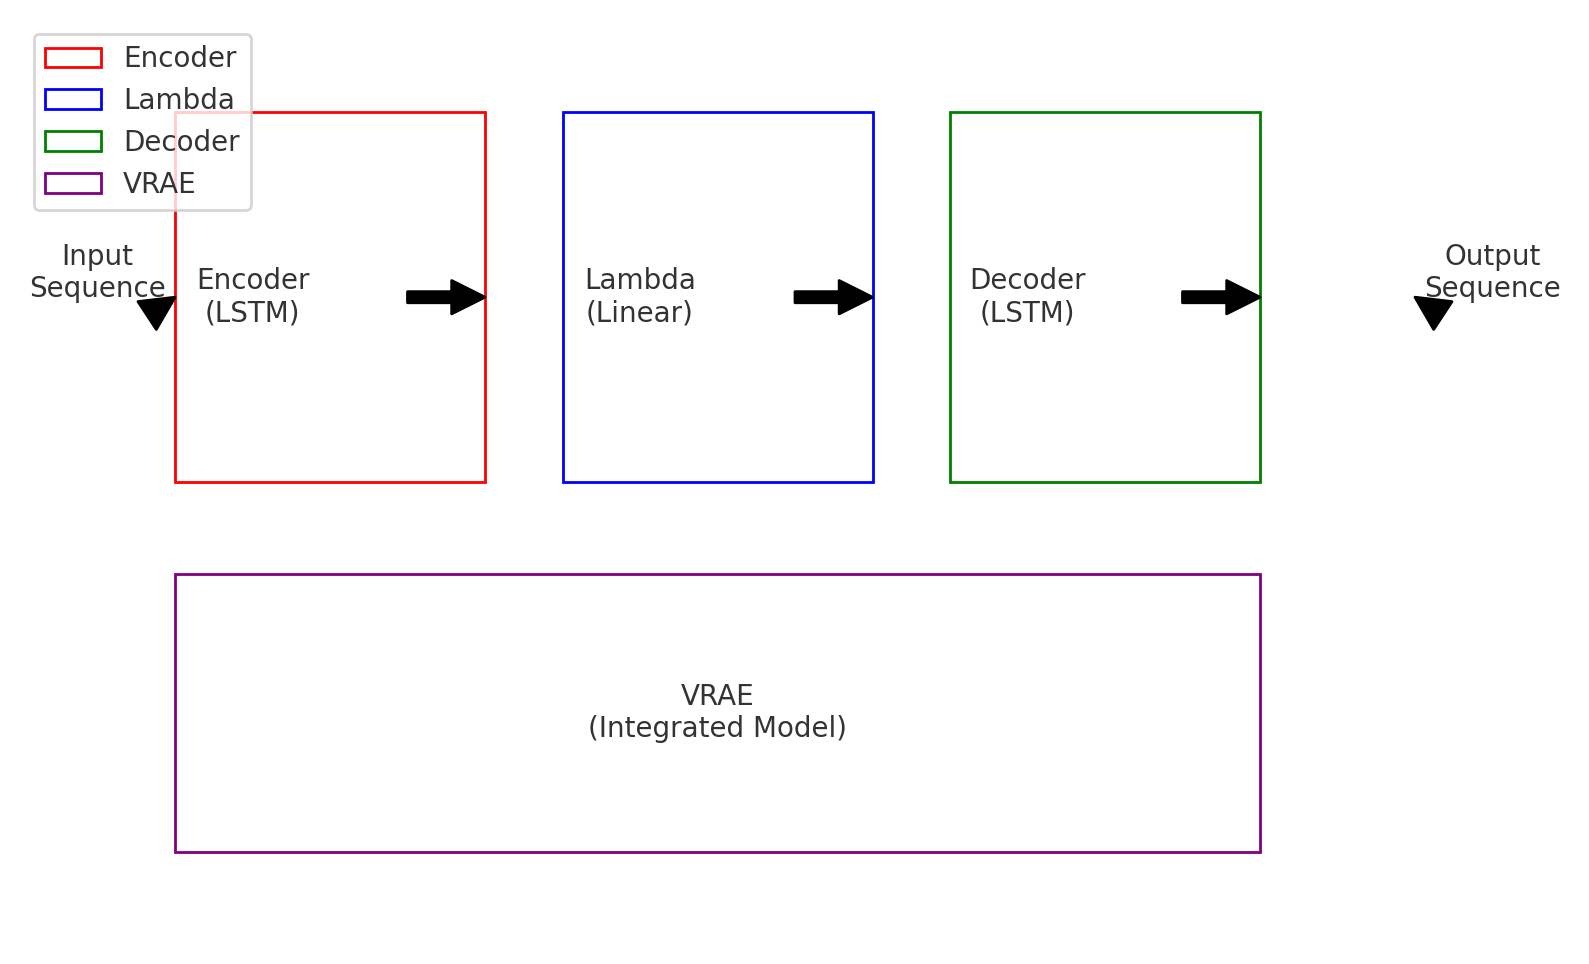
\includegraphics[scale=0.5]{cs236.png}

\begin{itemize}
    \item Encoder: Represented by the red box on the left, it takes the input sequence and passes it through LSTM layers to produce a hidden state.
    \item Lambda: Shown in blue, this module takes the hidden state from the Encoder and transforms it into a latent mean and log variance. It also includes a mechanism for sampling from the latent space during training.
    \item Decoder: Indicated by the green box, it takes the latent vector from the Lambda module and decodes it through LSTM layers to reconstruct the output sequence.
    \item VRAE: The purple box encompasses the whole architecture, highlighting how the VRAE integrates the Encoder, Lambda, and Decoder components.
\end{itemize}


\section{Preliminary Results}

For the progress report, we mainly focused on training a variational autoencoder to learn a good latent space for the EEG scans. 

After normalizing and pre-processing all of the data, we achieve a loss of ~1130 for VRAE and a loss of around ~1047 for a vanilla VAE (1-D convolutional layers):

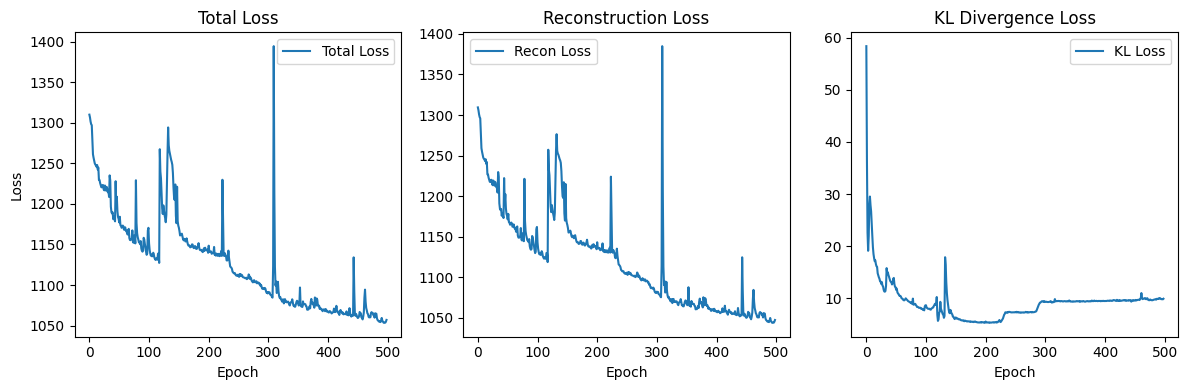
\includegraphics[scale = 0.5]{cs236b.png}

We then used t-SNE to visualize (high-dimensional, not 2) the latent space vectors belonging to the first 5 classes ($5 \times 10$ images, so $50$ encoded latent EEG scans). For reference, the first ten latent vectors should be clustered close together, the second ten should be another cluster, and so on. However, this was not the case in preliminary results: 

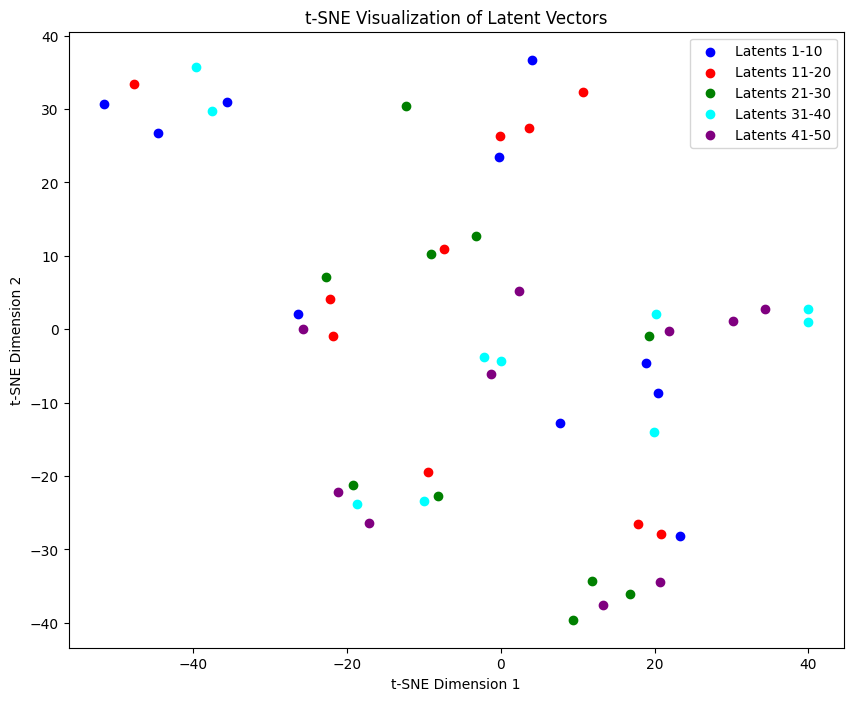
\includegraphics[scale=0.5]{cs236c.png}

To further explore this issue, we applied K-means clustering to the latents array with $n_{clusters} = 2$ to see if there was a possibility to derive some sort of relationship between our encoded EEG scans (latents) and corresponding classes. However, this was also not the case. K-means was close to random (every ten latents (1:10, 11:20, 21:30, ...) should be under same cluster, but it was not), and to see this, we printed out the labels of the first ten latents: [1, 0, 1, 0, 0, 1, 0, 1, 0, 0]. See that under $n_{clusters} = 2$, to have a four-five split for the first ten latents (they should be under same cluster) is pretty bad. This result is also similar for the second ten latents, third, fourth, and so on.




\end{document}